\chapter{Introducción a matplotlib\\ Introduction to matplotlib}
\epigraph{El punto geométrico es invisible. De modo que lo debemos definir como un ente abstracto. Si pensamos en él materialmente, el punto se asemeja a un cero.
Cero que, sin embargo, oculta diversas propiedades «humanas». Para nuestra percepción este cero —el punto geométrico—está ligado a la mayor concisión. Habla, sin duda, pero con la mayor reserva.}{Vasili Kandinski, Punto y línea sobre plano}
\begin{paracol}{2}
    Visualizar los datos es fundamental para poder comprender y transmitir ideas e información en ciencias e ingeniería.
    Python tiene numerosas funciones gráficas que para mostrar muchos tipos de gráficos. Una de las librerías para visualizar datos de uso más extendido es \href{https://matplotlib.org/stable/}{matplotlib} a la que dedicamos este capítulo.
    \switchcolumn
    Visualising data is essential for understanding and conveying ideas and information in science and engineering.
    Python has numerous graphics functions for displaying many types of graphics. One of the most widely used data visualisation libraries is \href{https://matplotlib.org/stable/}{matplotlib} to which we dedicate this chapter.
    \switchcolumn
    Importaremos la biblioteca matplotlib de la siguiente manera
    \switchcolumn
    We can import matplotlib as follows:
\end{paracol}

\begin{minted}{python}
    import matplotlib as mpl
\end{minted}
\begin{paracol}{2}
    \paragraph{matplotlib.pyplot} es una colección de funciones que hacen que matplotlib funcione como MATLAB. Cada función de pyplot realiza algún cambio en una figura: por ejemplo, crea una figura, crea un área de trazado en una figura, traza algunas líneas en un área de trazado, decora el trazado con etiquetas, etc.

    En matplotlib.pyplot la figura se conserva a través de las llamadas a funciones, de modo que las funciones de trazado se ejecutan sobre los ejes actuales.
    \switchcolumn
        \paragraph{matplotlib.pyplot} is a collection of functions that make matplotlib work like MATLAB. Each pyplot function makes some change to a figure: for example, it creates a figure, creates a plot area in a figure, draws some lines in a plot area, decorates the plot with labels, etc.

        In matplotlib.pyplot the figure is preserved across function calls, so that the plotting functions are executed on the current axes.
\switchcolumn
Para crear gráficas usando Matplotlib necesitaremos una figura. Cada figura tiene un par (o más) de ejes y un área que es donde se dibujarán los puntos en el sistema de coordenadas que decidamos. Además podremos poner títulos, leyendas etc...

\switchcolumn

To create graphs using Matplotlib we will need a figure. Each figure has a pair (or more) of axes and an area which is where the points will be drawn in the coordinate system of your choice. In addition we can put titles, legends etc...

\switchcolumn

La manera más sencilla de crear una figura es empleando el método \texttt{figure} que creará una figura en la que posteriormente podremos añadir ejes, títulos y más cosas. Simplemente llamando a \texttt{figure} creamos un objeto de tipo figura, aunque también podemos darle de manera opcional parámetros como el tamaño, el color de fondo y más.

\switchcolumn
The easiest way to create a figure is to use the \texttt{figure} method which will create a figure to which we can later add axes, titles and more. Simply by calling \texttt{figure} we create an object of type figure, although we can also optionally give it parameters such as size, background colour and more.
\end{paracol}

\begin{paracol}{2}

\end{paracol}
\begin{minted}{python}
import matplotlib.pyplot as plt
fig = plt.figure(figsize=(2, 2), facecolor='lightskyblue',
                 layout='constrained')
fig =plt.figure            
\end{minted}

\section{Dibujar en 2D}
\begin{paracol}{2}
    La manera más sencilla de dibujar usando matplotlib.pyplot es mediante el método \texttt{plot}. A este método le pasaremos dos vectores con las coordenadas $x$ e $y$ de los puntos que queremos representar (evidentemente tendremos que asegurarnos de que tienen la misma longitud).

    Por ejemplo si generamos unos vectores de coordenadas como los siguientes $x=(0,2,-1,-2)$ e $y=(0,3,2,-4)$, y se los pasamos al método \texttt{plot} pyplot dibujará los puntos $(x,y)$ y los unirá con rectas, como puede verse en la figura \ref{fig:pyplot-simple}.
    \switchcolumn
        The easiest way to draw using matplotlib.pyplot is by using the \texttt{plot} method. To this method we will pass two vectors with the $x$ and $y$ coordinates of the points we want to represent (obviously we will have to make sure that they have the same length).  

            For example, if we generate coordinate vectors such as $x=(0,2,-1,-2)$ and $y=(0,3,2,-4)$, and pass them to the pyplot method, it will draw the points $(x,y)$ and join them with straight lines, as can be seen in the figure \ref{fig:pyplot-simple}.
        
\end{paracol}
\begin{minted}{python}
import numpy as np
import matplotlib.pyplot as plt

x=np.array([0, 2, -1, -2])
y=np.array([0, 3, 2, -4])
plt.figure
plt.plot(x,y)
\end{minted}
\begin{figure}[h]
    \centering
    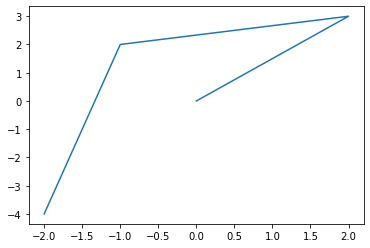
\includegraphics[width=0.5\linewidth]{figuras/pyplot01.png}
    \bicaption{Ejemplo sencillo de pyplot.} {Simple pyplot example.}
    \label{fig:pyplot-simple}
\end{figure}

\begin{paracol}{2}
    Además de las coordenadas de los puntos $(x,y)$ al método \texttt{pyplot.plot} podemos darle un tercer argumento indicando el formato (color y forma) con el que queremos que se grafiquen los puntos y opcionalmente la línea que los una. 

    Algunos de los colores y formatos admitidos están en las tablas \ref{tab:colores}, \ref{tab:puntos} y \ref{tab:lineas}. Para más información consulta la ayuda de \texttt{pyplot.plot}

    
    \begin{table}
        \centering
        \begin{tabular}{|c|c|} \hline
        \textbf{Símbolo}     &  \textbf{Color}\\
             'b'& azul \\ \hline
             'r'& rojo \\ \hline
             'g'& verde \\ \hline
             'm'& magenta\\ \hline
             'c'& cian\\ \hline
             'y'& amarillo\\ \hline
             'k'& negro\\ \hline
             'w'& blanco\\ \hline
        \end{tabular}
        \caption{Colores de los puntos}
        \label{tab:colores}
    \end{table}

    
    \begin{table}
        \centering
        \begin{tabular}{|c|c|} \hline
        \textbf{Símbolo}     &  \textbf{Formato punto}\\
             '.'& punto \\ \hline
             ','& píxel\\ \hline
             'o'& círculo \\ \hline
             's'& cuadrado\\ \hline
             '\^'& triángulo hacia abajo\\ \hline
             'v'& triángulo hacia arriba\\ \hline
             'p'& pentágono\\ \hline
             '*'& asterisco\\ \hline
        \end{tabular}
        \caption{Algunos de los marcadores de puntos}
        \label{tab:puntos}
    \end{table}

      \begin{table}
        \centering
        \begin{tabular}{|c|c|} \hline
        \textbf{Símbolo}     &  \textbf{Tipo de línea}\\
             '-'& sólida \\ \hline
             '--'& discontínua\\ \hline
             '-.'& punto-raya \\ \hline
             ':'& de puntos\\ \hline
        \end{tabular}
        \caption{Tipos de línea}
        \label{tab:lineas}
    \end{table}  
    \switchcolumn
    In addition to the coordinates of the points $(x,y)$, we can give the \texttt{pyplot.plot} method a third argument indicating the format (colour and shape) in which we want the points to be plotted and optionally the line that joins them. 

    Some of the colours and formats supported are in the tables \ref{tab:colours}, \ref{tab:dots} and \ref{tab:lines}. For more information, see the help for \texttt{pyplot.plot}.
    
    \begin{table}
        \centering
        \begin{tabular}{|c|c|} \hline
        \textbf{Symbol}     &  \textbf{Color}\\
             'b'& blue \\ \hline
             'r'& red \\ \hline
             'g'& green \\ \hline
             'm'& magenta\\ \hline
             'c'& cyan\\ \hline
             'y'& yellow\\ \hline
             'k'& black\\ \hline
             'w'& white\\ \hline
        \end{tabular}
        \caption{Point colors}
        \label{tab:colours}
    \end{table}

    
    \begin{table}
        \centering
        \begin{tabular}{|c|c|} \hline
        \textbf{Symbol}     &  \textbf{Point format}\\
             '.'& point \\ \hline
             ','& pixel\\ \hline
             'o'& circle \\ \hline
             's'& square\\ \hline
             '\^'& down triangle\\ \hline
             'v'& up triangle\\ \hline
             'p'& pentagon\\ \hline
             '*'& star\\ \hline
        \end{tabular}
        \caption{Some point markers}
        \label{tab:dots}
    \end{table}

      \begin{table}
        \centering
        \begin{tabular}{|c|c|} \hline
        \textbf{Symbol}     &  \textbf{Line type}\\
             '-'& solid \\ \hline
             '--'& dashed\\ \hline
             '-.'& dash and dot\\ \hline
             ':'& dotted\\ \hline
        \end{tabular}
        \caption{Line types}
        \label{tab:lines}
    \end{table}  
    
    \switchcolumn
    Se puede combinar un símbolo de cada tipo en un mismo \texttt{plot}. Así por ejemplo si queremos representar los datos anteriores unidos mediante una línea de puntos,
\begin{minted}{python}
plt.plot(x,y,':')    
\end{minted}

Si queremos que pinte solo los puntos sin unirlos con líneas y en color rojo,
\begin{minted}{python}
plt.plot(x,y,'.r')
\end{minted}

Si queremos que pinte los puntos representados por triángulos con el vértice hacia arriba, unidos mediante una línea continua y en color negro,

\begin{minted}{python}
plt.plot(x,y,'-^k')
\end{minted}

\switchcolumn
It is possible to combine one symbol of each type in the same text. So for example if we want to represent the above data joined by a dotted line,
\begin{minted}{python}
plt.plot(x,y,':')    
\end{minted}

If we want it to paint only the dots without joining them with lines and in red,
\begin{minted}{python}
plt.plot(x,y,'.r')
\end{minted}
If we want it to paint the points represented by triangles with the vertex upwards, joined by a continuous line and in black,

\begin{minted}{python}
plt.plot(x,y,'-^k')
\end{minted}


\switchcolumn
La figura \ref{fig:tplot} muestra los resultados de las combinaciones de símbolos que acabamos de describir.

\switchcolumn
Figure \ref{fig:tplot} shows the results of the symbol combinations just described.
\end{paracol}

\begin{figure}
    \centering
    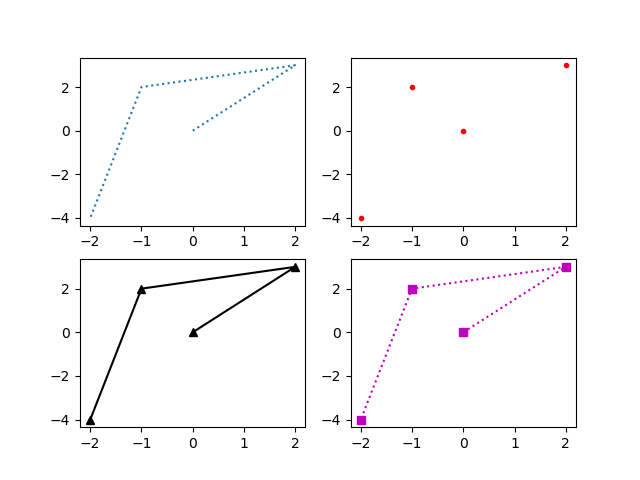
\includegraphics[width=1\linewidth]{figuras/tipos_plot.png}
    \bicaption{Ejemplos de dibujos con diferente formato}{Different uses of plot}
    \label{fig:tplot}
\end{figure}

\begin{paracol}{2}
    \paragraph{Scatter.} También podemos dibujar los puntos $x$, $y$, por separado sin unirlos usando el método \texttt{scatter(x,y)}. 
    \switchcolumn
    \paragraph{Scatter.} We can also draw the points $x$, $y$, separately without joining them using the method \texttt{scatter(x,y)}. 
\end{paracol}

\begin{paracol}{2}
\subsection{Trabajar con múltiples figuras}
Con \texttt{matplotlib.pyplot} se pueden dibujar diferentes gráficas en una misma figura usando el método \texttt{subplot}. Con este méotod crearemos una figura donde las distintas gráficas estarán dispuestas a modo de tabla. A este método le indicaremos mediante parámetros de entrada el número de filas, el número de columnas y la posición donde se va a dibujar la siguiente gráfica.

En el siguiente ejemplo se crean dos gráficas dentro de la misma figura en dos filas y una columna. En la primera se dibuja la gráfica del coseno y en la segunda la del seno. El resultado puede verse en la figura \ref{fig:subplot_01}.

\begin{minted}{python}
import numpy as np
import matplotlib.pyplot as plt
t1 = np.arange(0.0, 5.0, 0.1)
plt.subplot(2,1,1)
plt.plot(t1,np.cos(t1),'r.-')
plt.subplot(2,1,2)
plt.plot(t1,np.sin(t1),'b.-')
\end{minted}

\switchcolumn

\subsection{Working with multiple figures}
With \texttt{matplotlib.pyplot} you can draw different graphs in the same figure using the \texttt{subplot} method. With this method we will create a figure where the different graphs will be arranged as a table. To this method we will indicate by means of input parameters the number of rows, the number of columns and the position where the next graph is going to be drawn.

In the following example, two graphs are created within the same figure in two rows and one column. In the first one the cosine graph is drawn and in the second one the sine graph is drawn. The result can be seen in figure \ref{fig:subplot_01}.

\begin{minted}{python}
import numpy as np
import matplotlib.pyplot as plt
t1 = np.arange(0.0, 5.0, 0.1)
plt.subplot(2,1,1)
plt.plot(t1,np.cos(t1),'r.-')
plt.subplot(2,1,2)
plt.plot(t1,np.sin(t1),'b.-')
\end{minted}
\end{paracol}

\begin{figure}
    \centering
    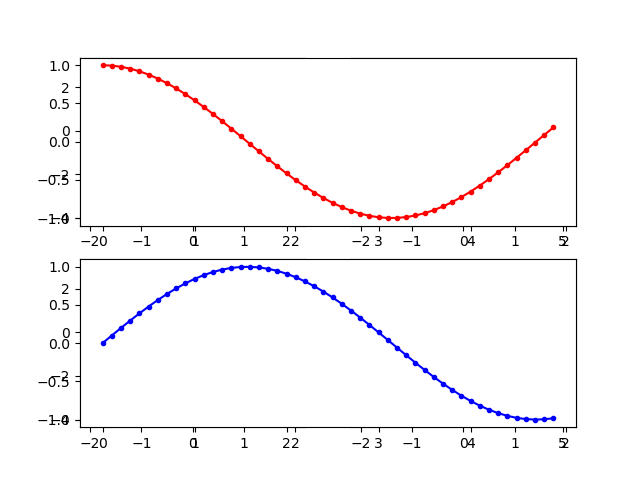
\includegraphics[width=0.75\linewidth]{figuras/subplot_01.png}
    \bicaption{Dos gráficas en una misma figura usando  \texttt{subplot}}{Two graphs in one figure using \texttt{subplot}}
    \label{fig:subplot_01}
\end{figure}

\begin{paracol}{2}
    Se puede añadir texto en cualquier parte del dibujo mediante el método \texttt{text} indicando las coordenadas donde se quiere poner el texto y el texto deseado. También se puede poner un texto como título de la figura, usando \texttt{title}, o etiquetando los ejes con \texttt{xlabel}, \texttt{ylabel}.

Por ejemplo el siguiente código da lugar a la figura \ref{fig:plot_text}.
  
\switchcolumn
Text can be added anywhere on the drawing using the \texttt{text} method, indicating the coordinates where the text is to be placed and the desired text. You can also put a text as the title of the figure, using \texttt{title}, or by labelling the axes with \texttt{xlabel}, \texttt{ylabel}.

For example, the following code results in the following figure \ref{fig:plot_text}.
 
\end{paracol}
 \begin{minted}{python}
import numpy as np
import matplotlib.pyplot as plt
plt.figure()
t=np.arange(0.0,5,0.01)
y=np.exp(-t) * np.cos(2*np.pi*t)
plt.plot(t,y)
plt.title("Evolución de un sistema amortiguado")
plt.xlabel('t(s)')
plt.ylabel('x(m)')
plt.text(2.5,0.8,'$x=e^{-t}\cos(2\pi \cdot t)$')
    \end{minted}
    
    \begin{figure}
    \centering
    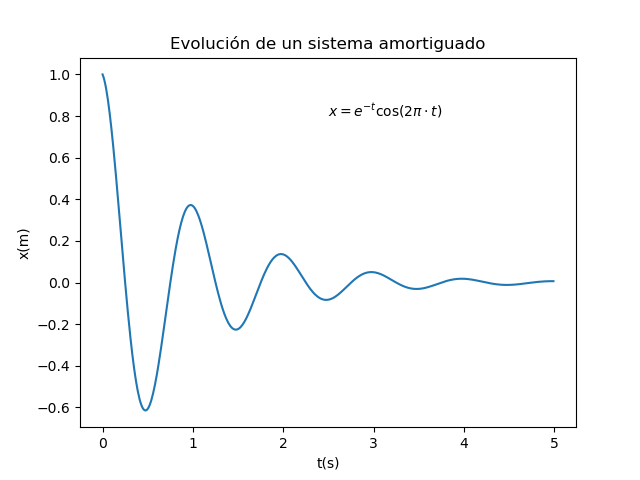
\includegraphics[width=0.75\linewidth]{figuras/plot_text.png}
    \bicaption{Figura con texto en etiquetas}{Figure with text and labels}
    \label{fig:plot_text}
\end{figure}
\begin{paracol}{2}
\subsection{Ejes no lineales}
    \texttt{Matplotlib.pytplot} cuenta con un método para definir la escala de los ejes, son los métodos \texttt{xscale} e \texttt{yscale}. Estos métodos pueden recibir como argumento el tipo de escala del eje, a elegir entre los siguientes:
    \begin{itemize}
        \item \texttt{"linear"} para definir una escala lineal
        \item \texttt{"log"} para definir una escala logarítmica de eje positivo
        \item \texttt{"symlog"} para definir una escala logarítmica con tramo positivo y negativo centrado en el cero (como los valores del logaritmo en torno al cero tienden a infinito hay una zona en torno al cero donde considera la escala lineal)
        \item \texttt{"logit"} escala logarítmica entre $0$ y $1$
    \end{itemize}
    Tanto \texttt{xscale} como \texttt{yscale} permiten definir la escala mediante una función que le definamos nosotros.

    En el siguiente ejemplo de código puede verse un ejemplo de uso de los métodos \texttt{xscale} e \texttt{yscale} para generar la figura \ref{fig:scale}.  
    
    Como se ve en la figura \ref{fig:scale}  las divisiones del eje logarítmico (eje y en la segunda figura y ambos en la tercera) aparecen marcadas como potencias de 10. Como estamos representando empleando el logaritmo decimal de la variable, las divisiones se corresponden con el exponente de la potencia de 10 de cada división, $\log_{10}(10^n)=n$.
    
    En segundo lugar hemos empleado un nuevo método: \texttt{grid()}. Este método añade una retícula al gráfico de modo que sea más fácil ver los valores que toman las variables en cada punto de la gráfica. Si se invoca el método \texttt{grid()} sin parámetros cambia la retícula de visible a invisible y viceversa.


    \switchcolumn
    \subsection{Nonlinear axis}
    \texttt{Matplotlib.pytplot} has a method to define the scale of the axes, these are the methods \texttt{xscale} and \texttt{yscale}. These methods can take as an argument the scale type of the axis, choose from the following:
    \begin{itemize}
        \item ‘linear’ to define a linear scale
        \item \texttt{‘log’} to define a positive-axis logarithmic scale
        \item \texttt{‘symlog’} to define a logarithmic scale with a positive and negative span centred at zero (as the values of the logarithm around zero tend to infinity there is a zone around zero where the linear scale is considered)
        \item{‘logit’} logarithmic scale between $0$ and $1$.
    \end{itemize}
    Both \texttt{xscale} and \texttt{yscale} allow the scale to be defined by a function that we define.

    The following code example shows an example of using the \texttt{xscale} and \texttt{yscale} methods to generate the \ref{fig:scale} figure.  
    
    As can be seen in the figure \ref{fig:scale} the divisions of the logarithmic axis (y-axis in the second figure and both in the third figure) are marked as powers of 10. As we are representing using the decimal logarithm of the variable, the divisions correspond to the exponent of the power of 10 of each division, $\log_{10}(10^n)=n$.

    Secondly, we have employed a new method: \text{grid()}. This method adds a grid to the graph so that it is easier to see the values taken by the variables at each point on the graph. Calling the \texttt{grid()} method without parameters toggles the visibility of the grid.
\end{paracol}
\begin{minted}{python}
import numpy as np
import matplotlib.pyplot as plt
x=np.linspace(0,10,100)
y=np.exp(x)
plt.figure()

plt.subplot(3,1,1)
plt.plot(x,y)
plt.grid()
plt.xlabel("Escala lineal")
plt.ylabel("Escala lineal")
plt.title("$y=e^x$")

plt.subplot(3,1,2)  
plt.plot(x,y)
plt.yscale('log')
plt.xlabel("Escala lineal")
plt.ylabel("Escala logarítmica")
plt.grid()


plt.subplot(3,1,3)  
plt.plot(x,y)
plt.xscale('log')
plt.yscale('log')
plt.xlabel("Escala logarítmica")
plt.ylabel("Escala logarítmica")
plt.grid()

\end{minted}

\begin{figure}[h]
    \centering
    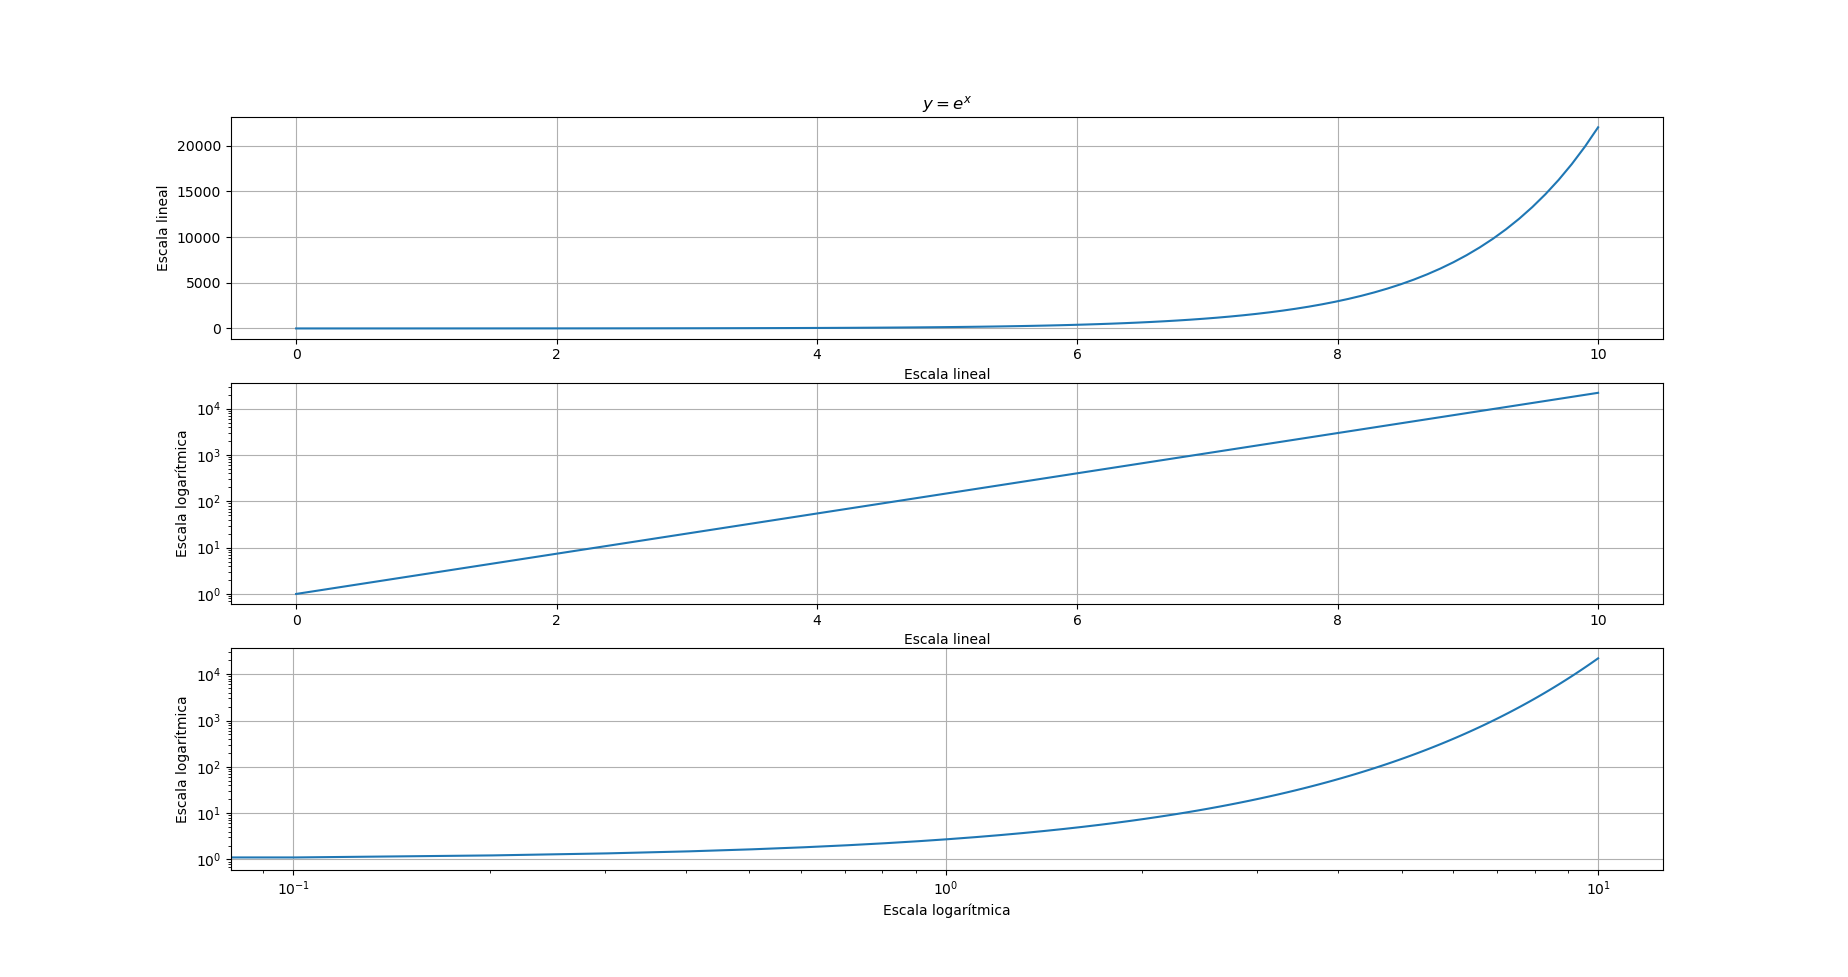
\includegraphics[width=1\linewidth]{figuras/plt_log_scales.png}
    \bicaption{Gráfica de la función $y=e^x$ con ejes en escala lineal y logarítmica}{Graph of the function $y=e^x$ with axes on linear and logarithmic scale}
    \label{fig:scale}
\end{figure}
\begin{paracol}{2}
\subsection{Gráfica en coordenadas polares}
Usando el método \texttt{polar} podemos representar funciones en coordenadas polares. El primer argumento  es un ángulo en radianes y el segundo el correspondiente radio. La figura \ref{fig:sp} muestra la espiral,

\begin{equation*}
r=2\cdot\sqrt{\theta}
\end{equation*}

Para el intervalo angular $[0,8\pi]$.

 \switchcolumn

\subsection{Polar coordinates graph}
Using the \texttt{polar} method we can plot functions in polar coordinates. The first argument is an angle in radians and the second the corresponding radius. The figure \ref{fig:sp} shows the spiral,

\begin{equation}
r=2\cdot\sqrt{\theta}
\end{equation}

For the angular interval $[0,8\pi]$.
\end{paracol}
\begin{minted}{python}
import numpy as np
import matplotlib.pyplot as plt

theta=np.linspace(0,8*np.pi,100)
radio=2*theta
plt.figure()
plt.polar(theta,radio,'b.-')
plt.grid(visible=True)
plt.title("Espiral en polares")
\end{minted}

\begin{figure}[h]
    \centering
    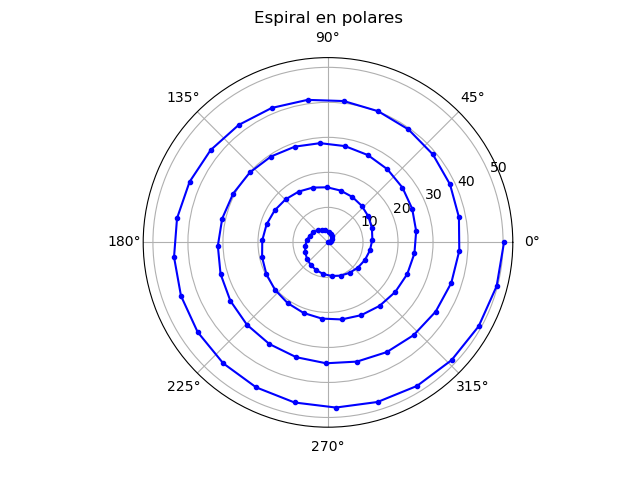
\includegraphics[width=0.75\linewidth]{figuras/plt_polar.png}
    \bicaption{Espiral en coordenadas polares}{Spiral plot using polar coordinates}
    \label{fig:sp}
\end{figure}

\begin{paracol}{2}
    \subsection{Otras representaciones gráficas}
    Con \texttt{matplotlib.pyplot} tenemos más opciones para hacer otro tipo de representaciones gráficas.

    \paragraph{hist}. Este método permite dibujar el histograma de una colección de datos. El histograma representa cuántos datos de una colección caen dentro de un intervalo dado. El método \texttt{hist} necesita como parámetro de entrada un vector de datos. Si no se le indica otra cosa los datos se agrupan en $10$ intervalos. Si se quiere cambiar el número de intervalos se puede indicar con el parámetro \texttt{bin}. En el siguiente ejemplo se dibuja el histograma de los datos de coches por cada $1000$ habitantes usando el método \texttt{hist} con el número de intervalos por defecto, con $5$ intervalos y con $10$. Los datos se cargan de un fichero llamado \textit{coches.dat} y la figura \ref{fig:plt_hist} es la figura resultante.

    \switchcolumn
    \subsection{Other graphical representations}
    With \texttt{matplotlib.pyplot} we have more options to make other types of graphical representations.

    \paragraph{hist}. This method allows you to draw the histogram of a collection of data. The histogram represents how much data in a collection falls within a given interval. The \texttt{hist} method requires a vector of data as input parameter. Unless otherwise specified, the data is grouped into $10$ intervals. If you want to change the number of intervals you can specify it with the parameter \texttt{bin}. In the following example the histogram of the car data per $1000$ inhabitants is drawn using the \texttt{hist} method with the default number of intervals, with $5$ intervals and with $10$ intervals. The data is loaded from a file called \textit{cars.dat} and the resulting figure \ref{fig:plt_hist} is the resulting figure.
\end{paracol}

\begin{minted}{python}
import numpy as np
import matplotlib.pyplot as plt

# Abrir el archivo en modo lectura
with open('coches.dat', 'r') as file:
    lineas=file.readlines() 
    f=len(lineas)
    n=np.zeros([f])
    i=0
    for row in lineas:
        n[i]=float(row)
        i+=1


plt.figure()

plt.subplot(1,3,1)
plt.hist(n)
plt.grid(visible=True)
plt.title("10 intervalos")
plt.xlabel("Coches por cada 1000 habitantes")
plt.ylabel("Número de paises")
plt.subplot(1,3,2)
plt.hist(n, bins=5)
plt.grid(visible=True)
plt.title("5 intervalos")
plt.xlabel("Coches por cada 1000 habitantes")
plt.ylabel("Número de paises")
plt.subplot(1,3,3)
plt.hist(n,bins=20)
plt.grid(visible=True)
plt.title("20 intervalos")
plt.xlabel("Coches por cada 1000 habitantes")
plt.ylabel("Número de paises")
\end{minted}

\begin{figure}
    \centering
    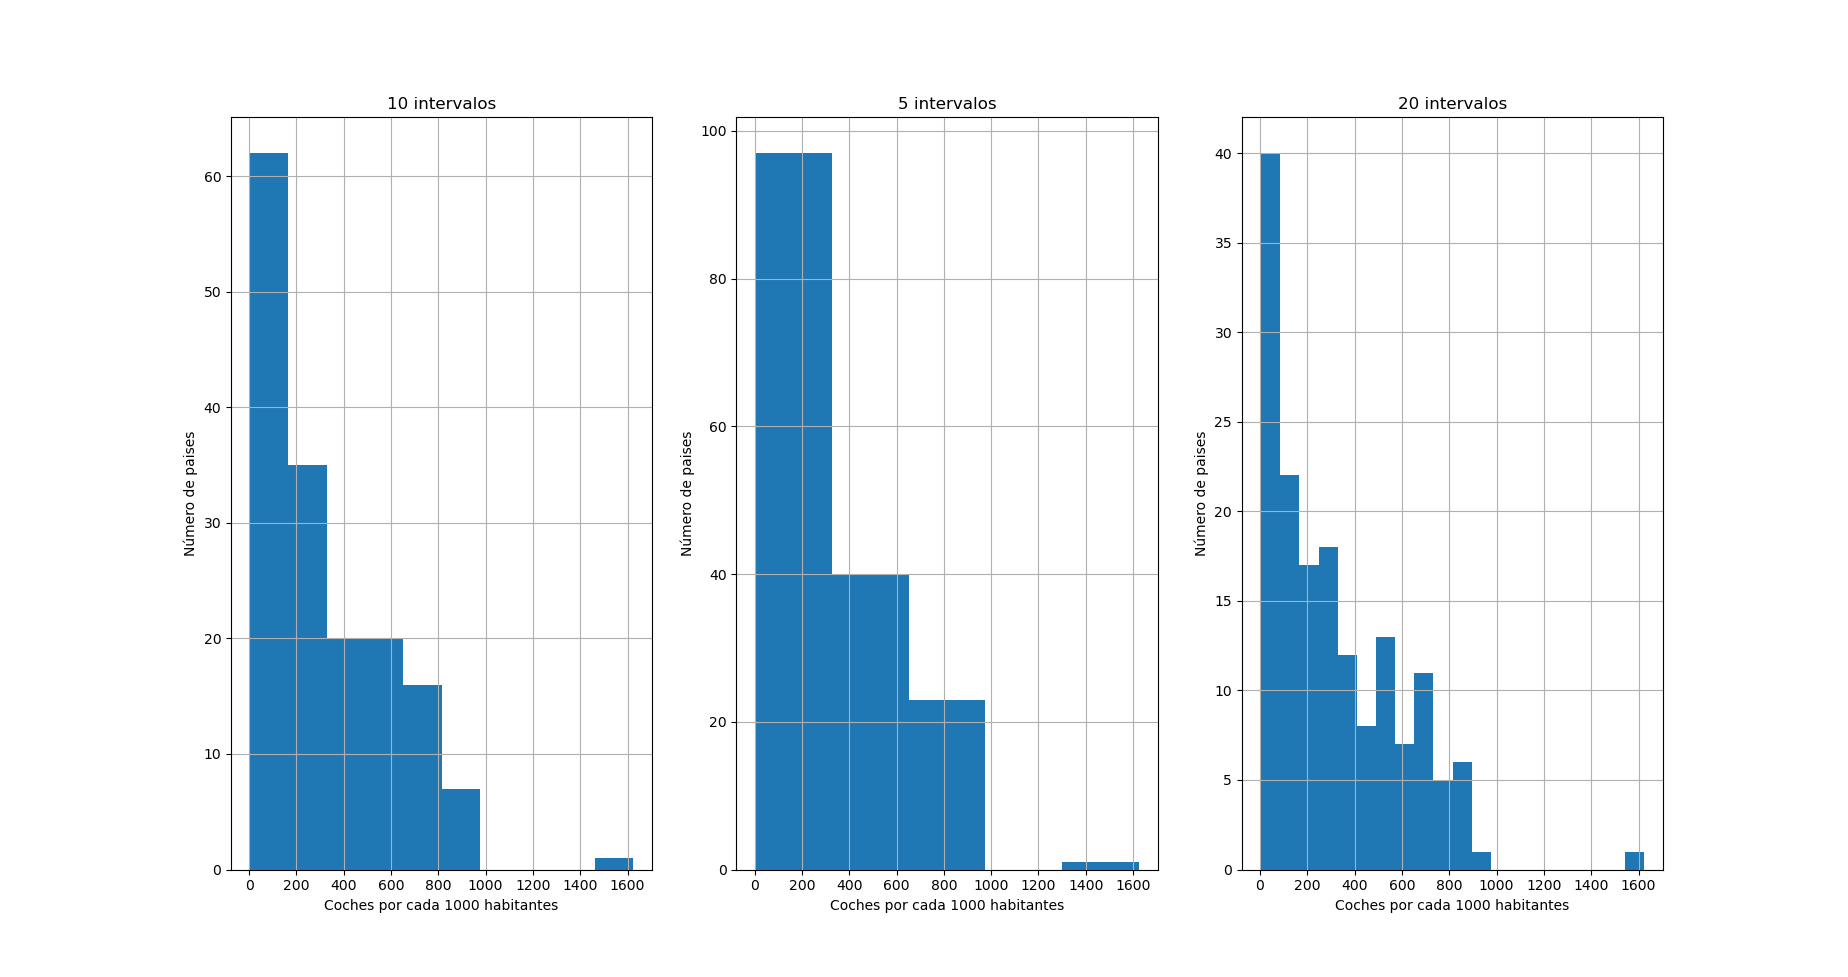
\includegraphics[width=1\linewidth]{figuras/plt_hist.png}
    \bicaption{Histogramas del número de automóviles por cada $1000$ habitantes}{}
    \label{fig:plt_hist}
\end{figure}

\begin{paracol}{2}
\section{Dibujar en 3D}
En tres dimensiones es posible representar dos tipos de gráficos: puntos y curvas, análogos a los representados en dos dimensiones y además superficies en el espacio.

\paragraph{subplots} Este método encapsula todo lo necesario para crear una figura y un conjunto de subfiguras contenidas en ella. Podemos indicarle muchos parámetros como el número de filas y de columnas de la rejilla de subfiguras, si se comparten o no los ejes entre ellas etc. También podemos indicar, mediante un diccionario qué tipo de proyección queremos usar en los ejes creados. Concretamente mediante el par clave-valor siguiente estamos indicando que queremos ejes en 3d  \textit{subplot\_kw="projection":"3d"}.

\switchcolumn
\section{3D plots}
In three dimensions it is possible to represent two types of graphics: points and curves, analogous to those represented in two dimensions, and also surfaces in space.

\paragraph{subplots} This method encapsulates everything needed to create a figure and a set of subfigures contained in it. We can indicate many parameters such as the number of rows and columns of the grid of subfigures, whether or not the axes are shared between them, etc. We can also indicate, by means of a dictionary, which type of projection we want to use in the axes created. Concretely, by means of the following key-value pair, we are indicating that we want 3d axes \textit{subplot\_kw=‘projection’: ‘3d’}. 


\end{paracol}

\begin{minted}{python}
    matplotlib.pyplot.subplots(nrows=1, ncols=1, *, sharex=False,
    sharey=False, squeeze=True, width_ratios=None, height_ratios=None, 
    subplot_kw=None, gridspec_kw=None, **fig_kw)
\end{minted}
\begin{paracol}{2}

Por ejemplo, podemos representar la curva,
\begin{align*}
y&=\sin(2\pi x)\\
z&=\cos(2\pi x)
\end{align*}

Para ello, seleccionamos un intervalo de valores para $x \in (0,2)$, y calculamos los correspondientes valores de $y$ y $z$. Los representamos usando el método \textit{scatter}, figura \ref{fig:3dscatter}.

\switchcolumn
For example, we can represent the curve,
\begin{align*}
y&=\sin(2\pi x)\\
z&=\cos(2\pi x)
\end{align*}

To do this, we select an interval of values for $x \in (0,2)$, and calculate the corresponding values of $y$ and $z$. Then, we plot them using the \textit{scatter} method, Figure \ref{fig:3dscatter}.

\end{paracol}

\begin{minted}{python}
import matplotlib.pyplot as plt
import numpy as np

x=np.linspace(0,2,100)
y=np.sin(2*np.pi*x)
z=np.cos(2*np.pi*x)

fig,ax=plt.subplots(subplot_kw={"projection": "3d"})
ax.scatter(x,y,z)  
\end{minted}


\begin{figure}
    \centering
    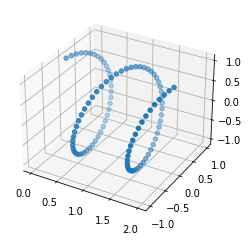
\includegraphics[width=0.5\linewidth]{figuras/scatter3d.png}
    \bicaption{Representación en 3 dimensiones usando \textit{scatter}}{3D plot using \textit{scatter}}
    \label{fig:3dscatter}
\end{figure}
\begin{paracol}{2}
\subsection{Superfícies}
Para dibujar una superfície emplearemos el método \textit{plot\_surface}. Igual que en el caso del método \textit{scatter} tendremos que crear previamente una figura y unos ejes en 3 dimensiones usando \textit{subplots} e indicando que se trata de una proyección en 3D.

Para poder dibujar una superfície con \textit{plot\_surface} hay que generar una rejilla $(X_m,Y_m)$ y en cada uno de los puntos de esa rejilla calcular el valor de la superfície.

Para definir dicha retícula  se necesitan dos matrices. Una de ellas $X_m$ contiene las coordenadas $x$ de los nodos de la retícula y la otra $Y_m$ las coordenadas $y$. Los elementos que ocupan la misma posición en ambas matrices, representan ---juntos--- un punto en el plano.

Matplotlib emplea dichas matrices como matrices de \emph{adyacencia}. Cada nodo, $(x_m(i,j),y_m(i,j)$, aparecerá en la gráfica conectado por una arista a cada uno de sus cuatros puntos vecinos, $(x_m(i-1,j),y_m(i-1,j)$, $(x_m(i,j-1),y_m(i,j-1)$, $(x_m(i+1,j),y_m(i+1,j)$, $(x_m(i,j+1),y_m(i,j+1)$.
Supongamos que empleamos las siguientes matrices, $X_m$ y $Y_m$ para definir una retícula sobre la que dibujar una superficie,

\switchcolumn

To draw a surface we will use the \textit{plot\-surface} method. As in the case of the \textit{scatter} method, we will have to previously create a figure and axes in 3 dimensions using \textit{subplots} and indicating that it is a 3D projection.

In order to draw a surface with \textit{plot\_surface} we must generate a grid $(X_m,Y_m)$ and at each of the points of this grid calculate the value of the surface.

To define such a grid, two matrices are needed. One of them $X_m$ contains the $x$ coordinates of the grid nodes and the other $Y_m$ the $y$ coordinates. Elements occupying the same position in both matrices represent - together - a point in the plane.

Matplotlib uses these matrices as adjacency matrices. Each node, $(x_m(i,j),y_m(i,j)$, will appear in the graph connected by an edge to each of its four neighbouring points, $(x_m(i-1,j),y_m(i-1,j)$, $(x_m(i,j-1),y_m(i,j-1)$, $(x_m(i+1,j),y_m(i+1,j)$, $(x_m(i,j+1),y_m(i,j+1)$.
Suppose we use the following matrices, $X_m$ and $Y_m$ to define a lattice on which to draw a surface,$z$.

\end{paracol}

\begin{align*}
X_m=\begin{pmatrix}
0&1&2&3\\ 
0&1&2&3\\
0&1&2&3\\
0&1&2&3
\end{pmatrix},& Y_m\begin{pmatrix}
0&0&0&0\\
1&1&1&1\\
2&2&2&2\\
3&3&3&3
\end{pmatrix}\xrightarrow[nodos]{posiciones}\begin{matrix}
(0,0)&-&(1,0)&-&(2,0)&-&(3,0)\\
\vert&&\vert&&\vert&&\vert\\ 
(0,1)&-&(1,1)&-&(2,1)&-&(3,1)\\
\vert&&\vert&&\vert&&\vert\\
(0,2)&-&(1,2)&-&(2,2)&-&(3,2)\\
\vert&&\vert&&\vert&&\vert\\
(0,3)&-&(1,3)&-&(2,3)&-&(3,3)
\end{matrix}
\end{align*}


\begin{minted}
Axes3D.plot_surface(X, Y, Z, *, norm=None, vmin=None, vmax=None, 
lightsource=None, **kwargs)
\end{minted}

\begin{paracol}{2}
La estructura de las matrices $X_m$ e $Y_m$ del ejemplo anterior, es la típica de las matrices de adyacencia de una retícula cuadrada; la matriz  $X_m$ tiene la filas repetidas y la matriz $Y_m$ tiene repetidas la columnas. En el ejemplo las matrices son cuadradas y definen una retícula de $4\times 4$ nodos. En general, podemos definir una retícula rectangular de $m\times n$ nodos. En este caso las matrices empleadas para definir la retícula tendrían dimensión $m\times n$.

Para dibujar con Matplotlib superficies podemos en primer lugar definir la retícula a partir de dos vectores de coordenadas empleando el método de numpy \texttt{meshgrid}. En el ejemplo que acabamos de ver, hemos empleado una retícula que cubre el intervalo, $x\in[0,3]$ e $y\in[0,3]$. para definirlo creamos los vectores,
\begin{minted}{pycon}
x=np.arange(0,4)

x
Out[23]: array([0, 1, 2, 3])

y=np.arange(0,4)

y
Out[25]: array([0, 1, 2, 3])
\end{minted}
\switchcolumn
The structure of the $X_m$ and $Y_m$ matrices in the previous example is typical of the adjacency matrices of a square lattice; the $X_m$ matrix has repeated rows and the $Y_m$ matrix has repeated columns. In the example the matrices are square and define a lattice of $4\times 4$ nodes. In general, we can define a rectangular lattice of $times n$ nodes. In this case the matrices used to define the lattice would have dimension $m\times n$.

To draw with Matplotlib surfaces we can first define the grid from two coordinate vectors using the numpy method \texttt{meshgrid}. In the example we have just seen, we have used a grid covering the interval, $x\in[0,3]$ and $y\in[0,3]$. To define it we create the vectors,
\begin{minted}{pycon}
x=np.arange(0,4)

x
Out[23]: array([0, 1, 2, 3])

y=np.arange(0,4)

y
Out[25]: array([0, 1, 2, 3])
\end{minted}
\switchcolumn
A continuación empleamos el método \texttt{meshgrid} para construir las dos matrices de adyacencia. Numpy se encargará de repetir las filas y columnas necesarias,


\begin{minted}{pycon}
    [Xm,Ym]=np.meshgrid(x,y)
Xm
Out[20]: 
array([[0, 1, 2, 3],
       [0, 1, 2, 3],
       [0, 1, 2, 3],
       [0, 1, 2, 3]])

Ym
Out[21]: 
array([[0, 0, 0, 0],
       [1, 1, 1, 1],
       [2, 2, 2, 2],
       [3, 3, 3, 3]])
\end{minted}


\switchcolumn

Next, we use the method \texttt{meshgrid} to construct the two adjacency matrices. Numpy will take care of repeating the necessary rows and columns,


\begin{minted}{pycon}
    [Xm,Ym]=np.meshgrid(x,y)
Xm
Out[20]: 
array([[0, 1, 2, 3],
       [0, 1, 2, 3],
       [0, 1, 2, 3],
       [0, 1, 2, 3]])

Ym
Out[21]: 
array([[0, 0, 0, 0],
       [1, 1, 1, 1],
       [2, 2, 2, 2],
       [3, 3, 3, 3]])
\end{minted}

\switchcolumn    
Una vez construidas las matrices de adyacencia, solo necesitamos una matriz de valores para $Z_m$. Si definimos por ejemplo,


\begin{minted}{pycon}
    Zm=np.zeros(np.shape(Xm))

Zm
Out[35]: 
array([[0., 0., 0., 0.],
       [0., 0., 0., 0.],
       [0., 0., 0., 0.],
       [0., 0., 0., 0.]])
\end{minted}

\switchcolumn
Once the adjacency matrices are constructed, we only need a matrix of values for $Z_m$. If we define for example,

\begin{minted}{pycon}
    Zm=np.zeros(np.shape(Xm))

Zm
Out[35]: 
array([[0., 0., 0., 0.],
       [0., 0., 0., 0.],
       [0., 0., 0., 0.],
       [0., 0., 0., 0.]])
\end{minted}

\switchcolumn
Podríamos representar la retícula plana de la figura \ref{fig:mesh}, empleando por ejemplo el comando \texttt{plot\_wireframe(Xm, Ym, Zm)}.

\switchcolumn
We could represent the flat grid of the figure \ref{fig:mesh}, using for example the command \texttt{plot\_wireframe(Xm, Ym, Zm)}.

\end{paracol}

\begin{figure}
    \centering
    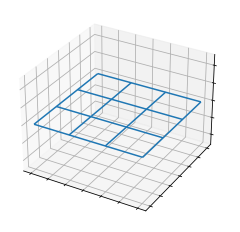
\includegraphics[width=0.5\linewidth]{figuras/reticula.png}
    \bicaption{Retícula plana}{Flat grid}
    \label{fig:mesh}
\end{figure}

\begin{paracol} {2}
Una vez que hemos visto como construir una retícula rectangular sobre la que construir una superficie, veamos como dibujarla con un ejemplo. Supongamos que queremos dibujar la superficie,
\begin{equation*}
z=x^3+y^2
\end{equation*}

En la región del plano, $x\in[-1.5,1.5]$, $y\in[-2,2]$. 
\switchcolumn
Now that we have seen how to construct a rectangular grid on which to build a surface, let's see how to draw it with an example. Suppose we want to draw the surface,
\begin{equation*}
z=x^3+y^2
\end{equation*}

In the region of the plane, $x\in[-1.5,1.5]$, $y\in[-2,2]$. 
\switchcolumn
Igual que en el ejemplo inicial, lo primero que debemos hacer es construirnos una matrices de adyacencia que definan una retícula en la región de interés,

\begin{minted}{pycon}
x=np.linspace(-1.5,1.5,25)
y=np.linspace(-2,2,50)
[Xm,Ym]=np.meshgrid(x,y)
\end{minted}

\switchcolumn
As in the initial example, the first thing to do is to construct adjacency matrices that define a grid in the region of interest,

\begin{minted}{pycon}
x=np.linspace(-1.5,1.5,25)
y=np.linspace(-2,2,50)
[Xm,Ym]=np.meshgrid(x,y)
\end{minted}

\switchcolumn

Es interesante notar que la región de interés no es cuadrada y que las matrices de adyacencia tampoco los son ($50\times 25$). Además los puntos no están espaciados igual en los dos ejes.

A continuación obtenemos la matriz de coordenadas z, aplicando la función a los puntos de la retícula,

\begin{minted}{pycon}
Zm=Xm**3+Ym**2
\end{minted}

\switchcolumn
It is interesting to note that the region of interest is not square and that the adjacency matrices are not square either ($50\times 25$). Also the points are not equally spaced on the two axes.

Next we obtain the z-coordinate matrix by applying the function to the grid points,

\begin{minted}{pycon}
Zm=Xm**3+Ym**2
\end{minted}

\switchcolumn
Podemos representar la superfície usando el método \textit{wireframe} o el método \textit{surface}. En el primer caso se dibuja la superfície como una rejilla, figura \ref{fig:wireframe} y en el segundo como las caras rellenas de color de la retícula, figura \ref{fig:surface}.

\switchcolumn

We can represent the surface using the \textit{wireframe} method or the \textit{surface} method. In the first case the surface is drawn as a grid, figure \ref{fig:wireframe}, and in the second as the colour-filled faces of the grid, figure \ref{fig:surface}.

\end{paracol}

\begin{figure}[h]
\centering
\subfigure[Función $z=x^3+y^2$ representada con \texttt{wireframe}\label{fig:wireframe}]{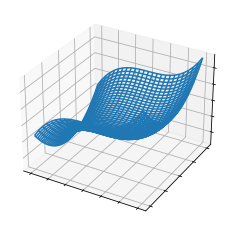
\includegraphics[width=8cm]{figuras/wireframe.png}} %\qquad 
\subfigure[Función $z=x^3+y^2$ representada con \texttt{surf} \label{fig:surface}]{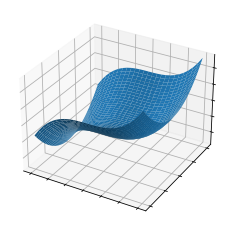
\includegraphics[width=8cm]{figuras/surface.png}}\\
\bicaption{Comparación entre \texttt{wireframe} y \texttt{surface}}{Comparison between \texttt{wireframe} and \texttt{surface}}
\end{figure}

\begin{paracol}{2}
\section{Animaciones}
Matplotlib también proporciona una interfaz para generar animaciones utilizando el módulo \textit{animation}. Una animación es una secuencia de fotogramas en la que cada fotograma corresponde a un trazado sobre una figura.

    \switchcolumn
    \section{Animations}
    Based on its plotting functionality, Matplotlib also provides an interface to generate animations using the \textit{animation} module. An animation is a sequence of frames where each frame corresponds to a plot on a figure.
    
\end{paracol}




\newpage
===============================================\\
he traído aquí el examen, porque aquí acababa antes el primer tema de programación\\
=================================================
\section{Test del curso 2020/21}
\begin{enumerate}

\item  El movimiento de un cuerpo en el plano viene descrito por las siguientes ecuaciones,

\begin{align}
x(t) &= \sin(2 \pi \, \omega_1 t)\\
y(t) &= \cos(2 \pi \, \omega_2 t)\\
z(t) &= a\cos(2\pi \, \omega_1 t) \label{eq:3}
\end{align}

donde $x,y,z$ representan las coordenadas del cuerpo en el instante de tiempo $t$ medidas en metros,  $w_1$ y $w_2$ son frecuencias fijas medidas en $rad\cdot s^{-1}$ y $a$ es una amplitud fija medida en metros.

\begin{enumerate}
	\item \label{ap1} (\textbf{1.5 puntos}) Escribe una función que:

\begin{enumerate}
	\item Tome como variables de entrada las frecuencias $w_1$, $w_2$, la amplitud $a$ .
	\item Haga el cálculo de la trayectoria en tres dimensiones descrita por el cuerpo en el intervalo de tiempo $[0,1]$. Considera incrementos de tiempo de $0.01s$.
	\item Dibuje en una gráfica la trayectoria descrita por el cuerpo en el espacio. Cada eje del gráfico deberá llevar  una etiqueta indicando de qué variable se trata $x$, $y$ ó $z$.
	\item La salida serán tres vectores con los valores de $x$, $y$ y $z$ calculados para cada instante de tiempo.
	\end{enumerate}

\item (\textbf{1.5 puntos}) Añade a la función creada en el apartado anterior el código necesario para que:
	\begin{enumerate}
	\item \textbf{Solo si} se le dan dos variables de entrada en lugar de tres, entonces calcule la trayectoria que describiría el cuerpo en el plano si se eliminara la ecuación (\ref{eq:3}) de las ecuaciones del sistema. (NOTA: La función debe seguir funcionando igual que en el apartado anterior si se le dan tres entradas. Emplea el comando nargin).
	\item El resultado deberá también representarse gráficamente, pero solo en dos dimensiones, y devolver la variable $z$ como un vector vacío. 
	\end{enumerate}

\item \label{ap2} (\textbf{1.5 puntos}) Crea un un \emph{live script} que genere dos  vectores de frecuencias: \texttt{W1} y \texttt{W2} de  modo que el primero contenga los números impares comprendidos entre $1$ y $7$ y el segundo los números pares comprendidos entres $2$ y $8$.  Emplea la función creada en el apartado anterior para calcular el valor de las trayectorias obtenidas tomando como entradas para  $\omega_1, \omega_2$,  todos los pares posibles de la forma: \texttt{W1(i)} y \texttt{W2(j)}. Supón que no hay tercera entrada $a$. Realiza los cálculos empleando bucles.

\item (\textbf{1 punto}) Añade a tu programa el código necesario para que dibuje cada resultado en un \emph{subplot} de modo que la figura resultante tenga $4\times4$ \emph{subplots} (ver figura al dorso).  Debes crear los \emph{subplots} empleando los mismos bucles del apartados anterior. 

\item (\textbf{0.5 puntos}) Repite los cálculos de los apartados c) y d) pero tomando ahora $a=1$.
\end{enumerate}

\item Una matriz cuadrada $A$, de dimensión arbitraria $(n\times n)$, cuyos elementos $a_{ij} \in \mathbb{Z}$, se define como \emph{buenrollista} cuando las suma de los valores pares de cada fila es mayor o igual que la suma de los valores  impares de la columna correspondiente, i.e., satisface la siguiente relación:
\begin{equation}
	\sum_{j=1}^n a_{ij\text{(par)}} \geq \sum_{j=1}^n a_{ji\text{(impar)}}, \quad \forall i\in\{1,...,n\}
\end{equation}

\begin{enumerate}
\item (\textbf{1.5 puntos}) Escribe  una función que tome como variable de entrada una matriz cuadrada de cualquier dimensión 
y calcule un vector con las sumas de los valores pares de los elementos de cada una de su filas  y otro vector con las sumas de los elementos impares de cada una de sus columnas.
\item (\textbf{1.5 puntos}) Añade a la función anterior el código necesario para que compruebe, empleando los vectores obtenidos en el apartado anterior, si la función es \emph{buenrollista} y muestre un mensaje por pantalla indicando si lo es o no.
\item (\textbf{1 punto}) Aplica la función desarrollada a la siguiente matriz:
\begin{equation*}
\begin{pmatrix}
2&3&4&6&1\\
5&4&-2&3&0\\
4&-1&5&4&-6\\
4&2&4&5&8\\
3&0&-3&-3&6
\end{pmatrix}
\end{equation*}
\end{enumerate}
\end{enumerate}
\noindent\rule{\textwidth}{0.4pt}
\begin{figure}[h]
\centering
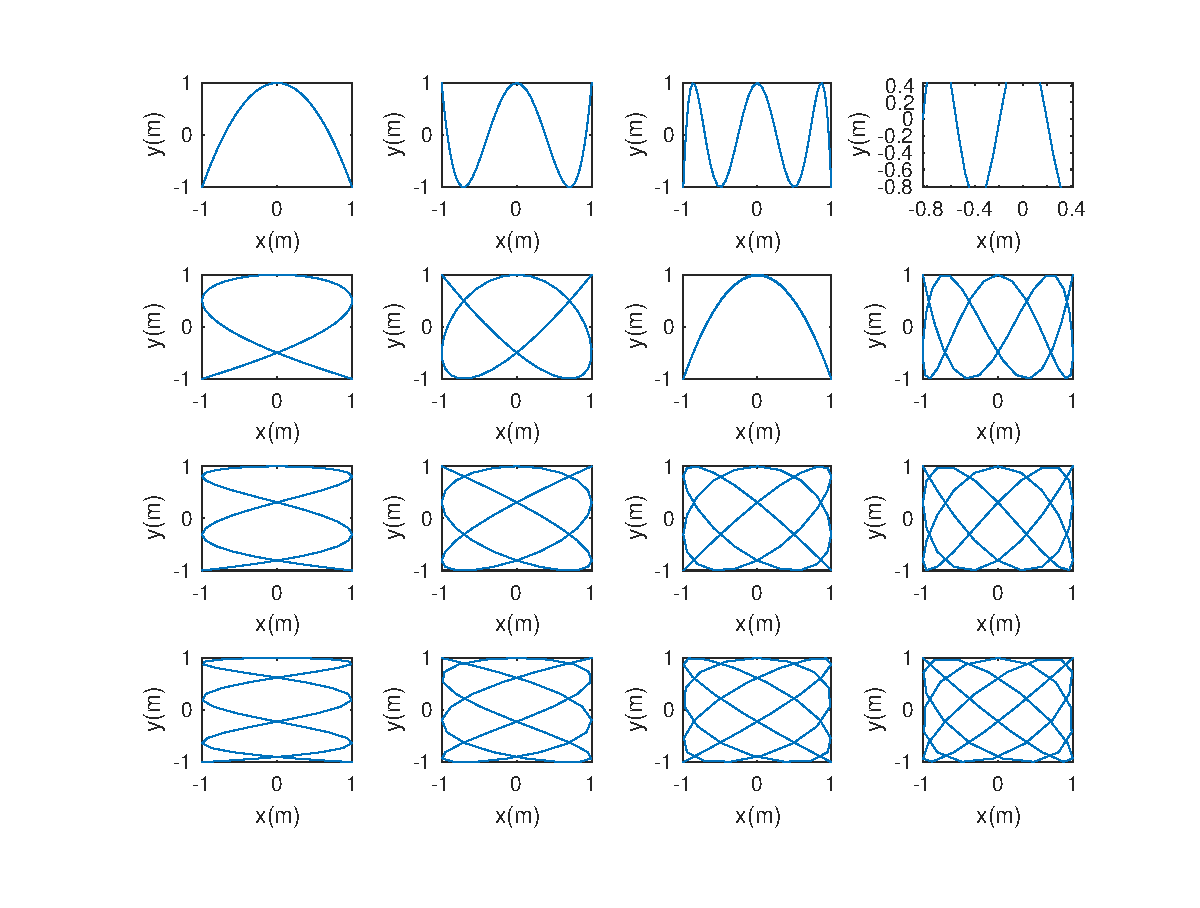
\includegraphics[scale=0.5]{lisa1.eps}
\caption{vista de la figura con los ocho subplots} \label{fig:1}
\end{figure}
